\subsection{Experiment Interfaces}

\subsubsection{Mechanical Interfaces}
\label{sec:4.2.1}

%\colorbox{orange}{\parbox{\textwidth}{THIS SECTION WILL BE FINALISED WHEN AN UPDATED CAD MODEL AND INTERFACE DESIGN WILL BE AVAILABLE}}\\

The experiment mounting platform will be attached to the lower rails of the gondola.

% Discuss mounting safety


\begin{figure}[H]
    \centering
	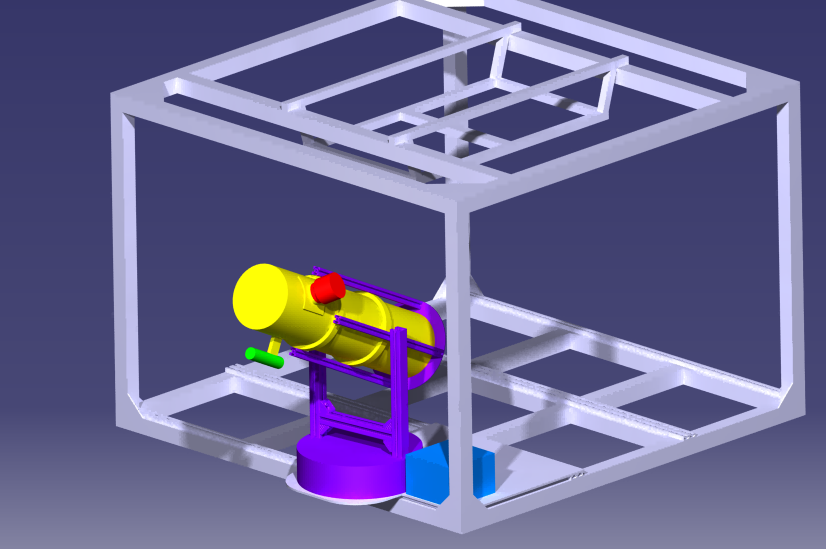
\includegraphics[width=0.9\linewidth]{4-experiment-design/img/mechanical/Assembly_v3iso2.png}
	\caption{Instrument position on gondola}
\end{figure}


% \bigskip
% \input{4-experiment-design/tables/attaching_comp.tex}


\subsubsection{Thermal Interfaces}

%\colorbox{orange}{\parbox{\textwidth}{THIS SECTION REQUIRES THERMAL ANALYSIS AND DESIGN}}\\

The IRISC experiment will be shielded from heat sources that could potentially introduce noise to the measurements. Once the final selection of components is made, Finite Element Analysis will be used to optimize the configuration of the components to ensure a good system performance.

\label{sec:4.2.2}


\subsubsection{Electrical Interfaces}
\label{sec:4.2.3}
\textbf{E-link:}\\
The uplink will be used to send occasional commands to control the experiment. The downlink will be used to send science and housekeeping data to the ground station. The TCP/IP protocol will be used for both the uplink and the downlink. The communication overhead for the uplink and downlink are composed of the TCP header (maximum 480 bits), the IP header (maximum 480 bits) and the Ethernet frame (144 bits). This results in an overhead of roughly 5 to 10\,\%. The size of one command will at most be in the single digit kB range resulting in a maximum uplink bandwidth of 1\,kbit/s. The downlink is greater in size due to scientific data with a minimum bandwidth of 300\,kbit/s and a nominal bandwidth of 500\,kbit/s. See paragraphs "Interfaces" and "Data acquisition and storage" in section \ref{sec:4.8.2} for more detail regarding the downlink.

\textbf{Power:}\\

Placed on the outside of the experiment structure/housing, the experiment will have a 4 pin, male, box mount receptacle MIL–C-26482P series 1 connector with an 8-4 insert arrangement (MS3112E8-4P).


% I comment this out because of Tomas comment that poower in not an interface. Also removed the 1mA. 
% Power will be delivered to the electronics box from the provided 28.8 V (13 Ah) battery pack. Only one pack is required. The expected % minimum current is [\hl{TBD}], the average is [\hl{TBD}] and the maximum is [\hl{TBD}]. More details in \ref{sec:4.7}.

\textbf{Connectors:}\\

%\begin{figure}[H]
%    \centering
%	\includegraphics[width=0.2\linewidth]{4-experiment-design/img/interfaces/power_cables.jpg}
%	\caption{[\hl{PLACEHOLDER}] Position of power cable socket}
%	\label{fig:power_cables}
%\end{figure}
%
%\begin{figure}[H]
%    \centering
%	\includegraphics[width=0.2\linewidth]{4-experiment-design/img/interfaces/elink_cables.jpg}
%	\caption{[\hl{PLACEHOLDER}] Position of E-link cable socket}
%	\label{fig:elink_cables}
%\end{figure}

Info about power cables, their length/resistivity and thus power loss, their connection to gondola power relay.



\textbf{Connectors:}\\

\textbf{Protection:}\\

\textbf{Grounding:}\\


\subsubsection{Radio Frequencies (Optional)}



\raggedbottom
